\chapter{Beszédadatbázisok}

A fejezet bemutatja a jelenleg ingyenes, bárki által elérhető és a tanítás során használt beszédadatbázisokat. Egy beszédadatbázis előállítása bár ránézésre egyszerű feladatnak tűnik,
valójában komplex folyamat és sok munkát igényel. Egyes adatbázisokat beszédfelismerés céljából készítettek, másokat beszélőfelismerésre. Az előbbinél kontrollált körülmények előállítása, megfelelés egyes nyelvtani mérőszámoknak (fonémák, diádok egyenletes elosztása stb.), utóbbinál a nagyobb méret miatt az automatizmus szükségessége bonyolítja a feladatot, valamint mindkét esetben a szerzői jogok védelmére is ügyelni kell. (A dolgozatban a beszédadatbázis, beszédkorpusz és beszédadathalmaz ugyanarra vonatkozik.)

\section{Beszédadatbázisok}

\subsection{TIMIT}

A TIMIT beszédkorpuszt automatikus beszédfelismerő rendszerek fejlesztéséhez tervezték. 630 beszélőtől tartalmaz mintákat amerikai angol nyelven a 8 legelterjedtebb nyelvjárásban.
A TIMIT archívum tartalmaz egy TRAIN és egy TEST mappát, ezek tanításhoz és teszteléshez valók. Ezeken belül további, a dialektusok sorszámával (DR1, ..., DR8), azon belül a beszélő azonosítójával elnevezett könyvtárak találhatók. Egy beszélőhöz
10 db beszédminta tartozik 16 kHz-es NIST SPHERE fájlok formájában.


\begin{table}[!ht]
	\begin{tabular}{*4l} \toprule
		\bfseries Dialektus regió (DR) & \bfseries Férfi & \bfseries Nő & \bfseries Összesen \\ \midrule
		1                             & 31 (63\%)      & 18 (27\%)   & 49 (8\%)          \\
		\rowcolor{gray!10} 
		2                             & 71 (70\%)      & 31 (30\%)   & 102 (16\%)        \\
		3                             & 79 (67\%)      & 23 (23\%)   & 102 (16\%)        \\
		\rowcolor{gray!10} 
		4                             & 69 (69\%)      & 31 (31\%)   & 100 (16\%)        \\
		5                             & 62 (63\%)      & 36 (37\%)   & 98 (16\%)         \\
		\rowcolor{gray!10} 
		6                             & 30 (65\%)      & 16 (35\%)   & 46 (7\%)          \\
		7                             & 74 (74\%)      & 26 (26\%)   & 100 (16\%)        \\
		\rowcolor{gray!10} 
		8                             & 22 (67\%)      & 11 (33\%)   & 33 (5\%)          \\
		\bottomrule
		\hline
	\end{tabular}
	\centering
	\caption{A beszélők eloszlása dialektusok szerint.}
	\label{fig:timit-dialects}
\end{table}

A dialektus régiók a következők:

\begin{multicols}{2}
	\begin{itemize}
		\item DR1:  New England
		\item DR2:  Northern
		\item DR3:  North Midland
		\item DR4:  South Midland
		\item DR5:  Southern
		\item DR6:  New York City
		\item DR7:  Western
		\item DR8:  Army Brat (moved around)
	\end{itemize}
\end{multicols}

A NIST SPHERE formátum az elején definiál egy fix hosszú fejlécet, amit a hang bináris kódolása követ. Erre figyelni kell a hangfájlok beolvasásánál, Python esetében nem minden hangfeldolgozó könyvtár támogatja. Ilyen esetben kézzel el kell távolítani a fejlécet a fájlok elejéről. A hangfájlokhoz tartozik egy szöveges dokumentum ami az elhangzott szöveget és annak a wav fájlbeli helyét tartalmazza. Továbbá egy WRD fájl írja le a szavakat és egy PHN kiterjesztésű a fonémákat, illetve azok időbeni elhelyezkedését a wav fájlban.

A hangfájlokhoz tartozó egyéb fájlok beszédfelismerés szempontjából fontosak. Mivel én a beszédkorpuszt beszélőfelismerésre használtam, csak a hangfájlokra volt szükségem. A TEST mappában - mivel a TIMIT-et alapvetően beszédfelismeréshez tervezték - teljesen különböző beszélők vannak a TRAIN mappához képest, ezért a TRAIN mappabeli beszélőket kell felosztani tanításhoz és teszteléshez.

\subsection{CMU Arctic}

A CMU Arctic adathalmaz beszédszintézishez kapcsolódó kutatásokhoz tervezték. A beszédszintézis az emberi beszéd mesterséges, általában számítógéppel történő előállítása. Mivel akkoriban a publikusan elérhető beszédadatbázisok kis méretűek voltak, létrehozták a CMU Arcticot, ami több beszédadatbázis összessége. Egy adatbázis egy beszélőhöz tartozik és tartalmaz egyéb információkat is, mint a fonetikus kiejtés vagy a beszédjel egyes jellemzőit (pitchmark) tartalmazó fájlok.
\newline
\newline
Mivel a CMU Arctic felhasználási célja a beszédszintézis, a felvételek studió minőségűek, mentesek külső zajoktól és a beszélő által keltett zajoktól is.
\newline
\newline
Az egyes Arctic adatbázisok közel 1150 kb. 1-4 másodperces beszédmintából állnak. Az egy beszélőhöz tartozó mintákat két azonos elemszámú A és B csoportra osztották, amelyek fonetikailag kiegyensúlyozottak. Ez azt jelenti, hogy az adott beszédmintában található fonémák körülbelül ugyanakkora gyakorisággal fordulnak elő mint az átlagos társalgás közben az adott nyelven.
A beszédminták WAV fájlok formájában 32 kHz-en lettek mintavételezve. A felvételek öt beszélőtől tartalmaznak hangmintákat:
\newline
\begin{itemize}
	\item férfi általános amerikai angol akcentus
	\item női általános amerikai angol akcentus
	\item férfi kanadai angol akcentus
	\item férfi skót angol akcentus
	\item férfi indiai angol akcentus
\end{itemize}
\bigskip
A CMU Arctic tartalmaz egy listát az egyes beszélők által felolvasott szövegekkel.
Mivel ez egy mindenki által elérhető ingyenes beszédadatbázisnak készült és szabad szoftver licensszel rendelkezik, fontos szempont volt, hogy a felolvasott szövegek ne sértsenek szerzői jogokat. Emiatt a listán szereplő mondantok a legnagyobb ingyenes, szabadon felhasználható szövegkorpuszból, a Gutenberg Projectből származnak. A Guteberg Project célja szerzői jogokat nem sértő angol nyelvű könyvek gyűjtése és elérhetővé tétele.
\newline
\newline
A CMU Arctic eleinte 2,5 millió szóból és az azokat tartalmazó 168000 mondatból állt. Ezekből a FestVox beszédszintézis projekt segítségével kiválogattak 52000 olyan mondatot, amelyek kiejtése könnyű és hossza 5 és 15 szó közé esett. A Festvox ugyan tartalmaz kiejtési További szigorításként csak olyan szavak kerülhettek be, amelyek részei a CMUDICT lexikonnak, hogy elkerüljék az eltérő kiejtést.
\newline
\newline
Ezután a Festvox segítségével az 52000 mondatból kiválogatták a legnagyobb diád lefedettségű halmazt. A diád két egymás utáni félhang együtteseként előálló nyelvi egység, amely lefedettségének mértéke a beszédszintézis során előállított beszéd minősége miatt fontos. 

A kiválogatott részt kivéve egy újabb halmazt választottak ki, amelyek 668 és 629 mondatból álltak. Ezeket manuálisan átnézve tovább finomították.

\begin{table}[!ht]
	\begin{tabular}{*4l} \toprule
		\bfseries Arctic & \bfseries Automatikus fázis & \bfseries Kézi finomítás I. & \bfseries Kézi finomítás II. \\ \midrule
		A halmaz                             & 668      & 597   & 593          \\
		\rowcolor{gray!10} 
		B halmaz                             & 629      & 541   & 539        \\
		Összesen                             & 1297      & 1138   & 1132        \\
		\bottomrule
		\hline
	\end{tabular}
	\centering
	\caption{Arctic CMU automatikus és kézi fázisok.}
	\label{fig:arctic-phases}
\end{table}

A CMU Arctic diád lefedettsége 80\% és az előbbihez hasonlóan triád lefedettsége 14\%. Az előbbi megelőzi mint a TIMIT beszédkorpuszban lévő diád lefedettséget, utóbbiban viszont a TIMIT jobb a több (2343) mondat miatt.

\begin{table}[!ht]
	\begin{tabular}{*8l} \toprule
		\bfseries Corpus & \bfseries Mondat & \bfseries Szó & \bfseries Fonéma  & \bfseries \begin{tabular}{@{}l@{}} Fonéma \\ lefedettség \end{tabular}  & \bfseries \begin{tabular}{@{}l@{}} Diád \\ lefedettség \end{tabular}  & \bfseries \begin{tabular}{@{}l@{}} Triád \\ lefedettség \end{tabular} \\ \midrule
		TIMIT-all & 2342 & 20771 & 87819 & 100\% & 78,2\% & 19,4\% \\
		\rowcolor{gray!10} 
		Arctic & 1132 & 10045 & 39153 & 100\% & 79,6\% & 13,7\% \\
		\bottomrule
		\hline
	\end{tabular}
	\centering
	\caption{Arctic CMU vs. TIMIT.}
	\label{fig:arctic-vs-timit}
\end{table}

\subsection{LibriSpeech}

2015-ben már vizsgálták a hangoskönyvek beszédszintézishez való használatát és léteztek ilyen célú beszédadatbázisok, de nem volt automatikus beszédfelismerés céljára létrehozott, ingyenes, mindenki által elérhető beszédkorpusz. A LibriSpeech beszédfelismerő rendszerek tanítására és kiértékelésére készült. Tartalma a LibriVox projektből származik, amelynek célja szabadon terjeszthető hangfelvételek készítése ingyenes, közkinccsé vált könyvekről, és ezek közzététele bárki számára az interneten.
\newline
\newline
A projekt körülbelül 1000 órányi beszédet tartalmaz 16 kHz-en mintavételezve. Tartalmaz ezek mellett több előre tanított beszédfelismerő modellt és Kaldi szkripteket beszédfelismerő rendszerek készítéséhez.
\newline
\newline
Az előfeldolgozási fázisban a könyvek szövegét normalizálták; kis és nagybetűk helyett csak nagybetűket használtak, eltüntették az írásjeleket és a gyakori rövidítések helyett a teljes szavakkal helyettesítették. Ezután a hangmintákat felismertették a Kaldi \emph{gmm-decode-faster} dekóderével, amihez egy VoxCeleb adatbázison tanított modellt használtak.
\newline
\newline
Összemérték az előbbi modell által felismert szöveget az eredeti írással és azokat a részeket választották ki, ahol a kettő megegyezett. A hanganyagot legfeljebb 35 másodperces részekre tördelték minimum 0.5 másodperces szünetek mentén.
\newline
\newline
A következő fázisban egy fMMRl (HMM-alapú) modellel ismét összemérték a felismert szöveget a valódival. Ez okozott hamis pozitív eredményeket is, de az audioanyag mennyisége miatt elhanyagolható volt. Ez a fázis tehát 35 másodperces nagy valószínűséggel helyesen transzkriptált anyagokat tartalmazott.
\newline
\newline
A harmadik fázis ezeknek az apróbb szegmensekre tördelése volt, amit két módszerrel végeztek el. Tanítóadatok esetén minden olyan szünetnél tördeltek, ahol az legalább 0,3 másodperc hosszú volt. Tesztadatok esetén csak ott tördeltek, ahol ez a szünet egybeesett a mondat végével is.

\begin{table}[!ht]
	\begin{tabular}{*6l} \toprule
		\bfseries Részhalmaz & \bfseries Óra & \bfseries beszélő / perc & \bfseries \begin{tabular}{@{}l@{}} Férfi \\ beszélő \end{tabular}
		& \bfseries \begin{tabular}{@{}l@{}} Női \\ beszélő \end{tabular} & \bfseries \begin{tabular}{@{}l@{}} Összes \\ beszélő \end{tabular} \\ \midrule
		dev-clean & 5,4 & 8 & 20 & 20 & 40 \\
		\rowcolor{gray!10} 
		test-clean & 5,4 & 8 & 20 & 20 & 40 \\
		dev-other & 5,3 & 10 & 16 & 17 & 33 \\
		\rowcolor{gray!10} 
		test-other & 5,1 & 10 & 17 & 16 & 33 \\
		train-clean-100 & 100,6 & 25 & 125 & 126 & 251 \\
		\rowcolor{gray!10}
		train-clean-360 & 363,6 & 25 & 439 & 482 & 921 \\
		train-other-500 & 496,7 & 30 & 564 & 602 & 1166 \\
		\bottomrule
		\hline
	\end{tabular}
	\centering
	\caption{LibriSpeech részhalmazok.}
	\label{fig:librispeech-subset}
\end{table}
\bigskip
Az audiófelvételek válogatásához a LibriVox API segítségével szereztek információkat a felolvasóról,
hogy mely hangoskönyvekben olvastak fel milyen fejezeteket, a kapcsolódó referencia szövegeket pedig a Gutenberg Project és Internet Archiveból nyerték ki. A train, dev és test részhalmazok között fontos, hogy ne legyen átfedés, tehát ugyanaz az olvasó ne olvasson csak egyetlen halmazban ezek közül. Ehhez a válogatáson kívül további óvintézkedésként kivették a többszereplős fejezeteket és lefuttaták a LIUM beszélő szegmentáló toolkitet ennek detektálására.
\newline
\newline
A tanítóhalmazba válogatott részeket három részre osztották. Ezek egyenként 100, 360 és 500 órányi audiofelvételt tartalmaznak. Az első kettőbe automatikus módszerrel az amerikai angol akcentushoz hasonló részeket válogatták bele. Egy egyszerű a Wall Street Journal si-84 adatbázisán tanított akusztikus modellt használtak a LibriSpeechen beszédfelismerésre. Ezáltal meghatározták és rangsorolták a beszélőket a Word Error Rate (a modell által hibásan felismert szavak) szerint. Az alacsonyabb WER pontszámmal rendelkező olvasók a clean, a magasabbal az other részhalmazokba kerültek.

\subsection{VoxCeleb1} \label{voxceleb1}

A beszélőfelismerésre használt adatbázisok kontrollált körülmények között felvett audio anyagot tartalmaznak és kézzel válogatottak, emiatt kis méretűek. Kontrollált körülmény alatt értjük a studioban felvett, külső és belső zajoktól mentes hanganyagot. Ezek a valós körülmények közötti, azaz zajos környezetben elhangzó beszédfelismerést megnehezítik. A VoxCeleb készítői a beszélőfelismerő adabázisok automatikus létrehozására terveztek egy folyamatot és létrehozták, valamint ingyenesen elérhetővé tették a VoxCeleb beszédadatbázist, ami valós körülmények közötti hanganyagot tartalmaz.
\newline
\newline

\begin{table}[!ht]
	\begin{tabular}{*4l} \toprule
		\bfseries Név & \bfseries Körülmények & \bfseries Beszélők száma & \bfseries Minták száma \\ \midrule
		ELSDSR                             & Kontrollált & 22     & 198          \\
		\rowcolor{gray!10} 
		Forensic Comparison                & Telefonos   & 552   & 1264        \\
		SITW                           & Multimédia        & 299   & 2800        \\
		\rowcolor{gray!10} 
		VoxCeleb                           & Multimédia        & 1251   & 153516        \\
		\bottomrule
		\hline
	\end{tabular}
	\centering
	\caption{Beszédadatbázisok beszédfelismerés.}
	\label{fig:speaker-recognition-datasets}
\end{table}

\bigskip
A VoxCeleb több mint 100000 olyan beszédmintát tartalmaz 1251 hírességtől, amik YouTube videókból származnak. Az adatbázisban a nemek aránya kiegyensúlyozott (férfiak 55\%, nők 45\%), a beszélők különböző származásúak, korúak illetve eltérő akcentussal rendelkeznek. A beszéd általában publikus eseményekről származik, így a háttérzaj, egyéb beszélők és a felvevő eszköz minősége zajossá teszi azt.
\newline
\newline
Az adatbázis előállítása a következő módon történt:
\begin{itemize}
	\item A beszélő jelöltek kiválasztása:  Olyan hírességeket válogattak akik benne vannak a VGG adathalmazban, ami 2622 híres (interneten sokat keresett) ember arcát tartalmazza.
	\item YouTube videók letöltése: Letöltötték a kiválasztott emberekhez tartozó első 50 YouTube videót. A keresés az illető nevét és utána az \emph{interview} szót tartalmazta, hogy kiszűrjék a zeneszámokat, sportfelvételeket és minél nagyobb valószínűséggel beszéljenek benne.
	\item Arcdetektálás: Az egyes videókon egy HOG-alapú arc detektorral meghatározták az arcok helyét minden egyes frameben.
	\item Aktív beszélőazonosítás: Mivel egy videóban több arc is megjelenhet egyszerre vagy a beszélőt szinkronizálhatják, az éppen beszélő arc meghatározására illetve az utóbbit kiszűrésére szükség volt. A megoldás a SyncNet volt, egy olyan kétcsatornás CNN, ami képes megbecsülni a szájmozgás és a beszéd közötti korrelációt.
	\item Arcfelismerés: Végül egy a VGG Face adathalmazzal tanított CNN segítségével ellenőrizték, hogy a beszélő arc valóban a kérdéses személy-e.
\end{itemize}

\subsection{VoxCeleb2} \label{voxceleb2}

A VoxCeleb2 ugyanúgy beszélőfelismeréshez készített, de az előző verzióhoz képest jóval nagyobb, 6112 hírességtől tartalmaz 2442 órányi beszédet tartalmazó beszédadatbázis különböző nyelvű, korú és származású beszélőkkel.
\newline
\newline
Az adatbázis előállítási folyamatot az előzőhöz képest tovább bővítették.
\begin{itemize}
	\item Duplikátum detektálás: YouTube-on gyakran feltöltik ugyanazt a videót más url alatt különböző felhasználók. Egy a VoxCeleb1 adatbázison tanított konvolúciós hálózatot használtak jellemző kinyerésre, amellyel 1024 dimenziós vektorokkal reprezentálták a beszédmintákat. Egy beszélőre kiszámolták a vektorpárok közötti Euklideszi-távolságot és ahol ez kisebb volt mint 0,1 azokat azonosnak tekintették.
	\item Nemzetiség: A beszélők nemzetiségét a Wikipediáról gyűjtötték ki egy keresőrobottal (angolul webcrawler). Ezzel a módszerrel a 6112 beszélő közül 5689 nemzetiségét sikeresen azonosították. Ebből kiderült, hogy a VoxCeleb2 etnikailag sokkal diverzifikáltabb a VoxCeleb1-hez képest, mivel a VoxCeleb1 adatbázisban jelenlévő 36 nemzetiségnél jóval többet, 145-öt tartalmaz. Ugyanakkor az amerikai angolt beszélők aránya is sokkal kisebb, 29\% a VoxCeleb1-ben mért 64\%-hoz képest.
\end{itemize}

\begin{table}[!ht]
	\begin{tabular}{*3l} \toprule
		\bfseries Adatok & \bfseries VoxCeleb1 & \bfseries VoxCeleb2 \\ \midrule
		Beszélők száma   & 1251 & 6112 \\
		\rowcolor{gray!10} 
		Beszélők száma   & 1251 & 6112 \\
		Női beszélők száma & 561 & 2351 \\
		\rowcolor{gray!10}
		Férfi beszélők száma & 690 & 3761 \\
		Videók száma & 22496 & 150480 \\
		\rowcolor{gray!10}
		Beszédminták száma & 153516 & 1128246 \\
		Átlagos videó / beszélő & 18 & 25 \\
		\rowcolor{gray!10}
		Átlagos beszédminta / beszélő & 116 & 185 \\
		Átlagos beszédminta hossz & 8,2 & 7,8 \\
		\bottomrule
		\hline
	\end{tabular}
	\centering
	\caption{VoxCeleb1 vs. VoxCeleb2.}
	\label{fig:voxceleb1-vs-2}
\end{table}

\chapter{Neurális hálózat alapú beszélőfelismerő rendszerek}

Ebben a fejezetben bemutatom két ingyenes, neurális hálózaton alapú beszélőfelismerő rendszer működését.
Mindkét rendszer zárt halmazú beszélőfelismerésre képes. A tanítást és tesztelést a TIMIT és CMU Arctic beszédadatbázisokkal végeztem.

\section{Mérési környezet}

A mérésekhez a Google Colaboratoryt használtam, amely gépi tanulási kutatások és oktatás céljából felhő alapú környezetet biztosít. Hozzáférni Google fiókkal lehet, egy felhasználó egy virtuális gépet és egy Jupyter Notebookot kap. Választhatunk, hogy  a notebook a Python 2-es vagy 3-as verzióját támogassa, illetve, hogy CPU-n, GPU-n vagy TPU-n szeretnénk tanítani. A Tensor Processing Unit (TPU) a Google által fejlesztett gyorsító hardver egység Tensorflows tanításokhoz.
\newline
\newline
Az erőforrásokhoz fájlrendszert is kapunk. Ehhez hozzácsatolhatjuk a Google Drive fiókunkat, így elérhetjük a rajta tárolt adatokat. A notebookon keresztül elérjük a mögötte futó Linuxot is, lehet terminál parancsokat futtatni ha \emph{!} vagy \emph{\%} jelöléssel kezdjük a sort. Ez lehetővé teszi azt is, hogy pl. kisebb méretű dolgokat \emph{wget}tel töltsünk le vagy navigáljunk a fájlrendszerben, létrehozzunk új mappákat vagy töröljünk, áthelyezzünk fájlokat. Ugyan egyszerre több notebookot használhatunk, a fájlrendszer és a hardveres erőforrások ezek között megosztottak.

\subsection{Adatok előfeldolgozása}

Az előfeldolgozó szkript a TIMIT adatbázis esetében a hangmintákról eltávolítja a NIST Sphere fejlécet és a mondat előtti és utáni szüneteket. Ezután normalizálja a hangmintákat. A CMU Arctic esetében a hangminták alapból normalizálva vannak, ezért csak azonos méretűre kell vágni őket az egységes bemeneti dimenziók érdekében (ahogy a TIMIT esetében is).

\section{WaveNet classifier}

A \emph{WaveNet classifier} egy módosított WaveNet architektúra beszélőidentifikációhoz.

\subsection{WaveNet}

A WaveNet egy mély neurális hálózat audio hullámformák generálásához, amelyet a Google DeepMind publikált 2016-ban. Az ötletet az akkori felfedezések adták neurális autoregresszív generatív modellezés terén, amelyeket komplex eloszlások, például képek modellezésére használtak (van den Oord et al., 2016a;b). Ezt felhasználva audio hullámformák generálásában új eredményeket értek el.

\begin{itemize}
	\item Képes olyan természetes hangzású beszéd hullámformák generálására, amit korábban parametrikus vagy konkatenatív beszédszintézissel sosem értek el. 
	\item Az audio hullámformák generáláshoz szükséges nagy receptív mezőt hatékonyan, nyújtott kauzális konvolúciókkal implementálja.
	\item Ha a modellt a beszélők identitásával tanítják, képes új hangok generálására.
	\item A zene generálás és a beszédfelismerés terén is ígéretesnek bizonyult.
\end{itemize}

\subsubsection{Nyújtott kauzális konvolúció}

A modell autoregresszív, vagyis a kimenete korábbi időpillanatokban felvett értékeitől függ. Ez azért fontos, mert a WaveNet egy generatív modell. A generált hullámforma \emph{t}-edik időpillanatbeli értéke nem függhet jövőbeli értékektől. A kauzalitás legegyszerűbb implementációja ha legalább a \emph{kernel-1} méretű paddinget adunk a konvolúcióhoz.

\begin{figure}[!ht]
	\centering
	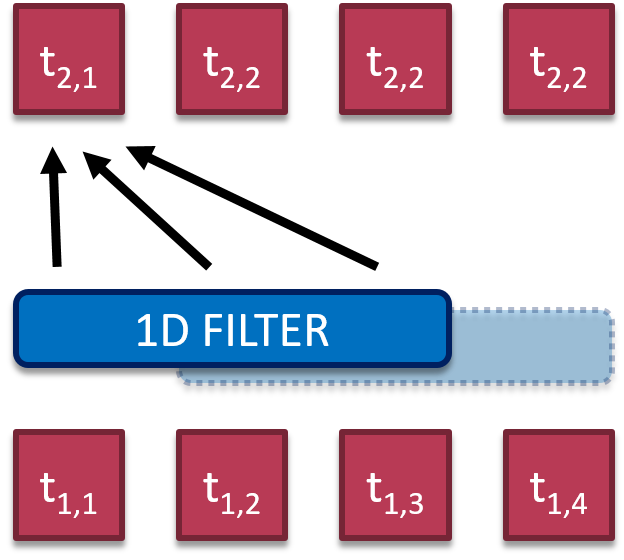
\includegraphics[width=80mm, keepaspectratio]{figures/1d-conv.png}
	\caption{1D nem kauzális konvolúció.}
	\label{fig:1d_noncausal_conv}
\end{figure}

\begin{figure}[!ht]
	\centering
	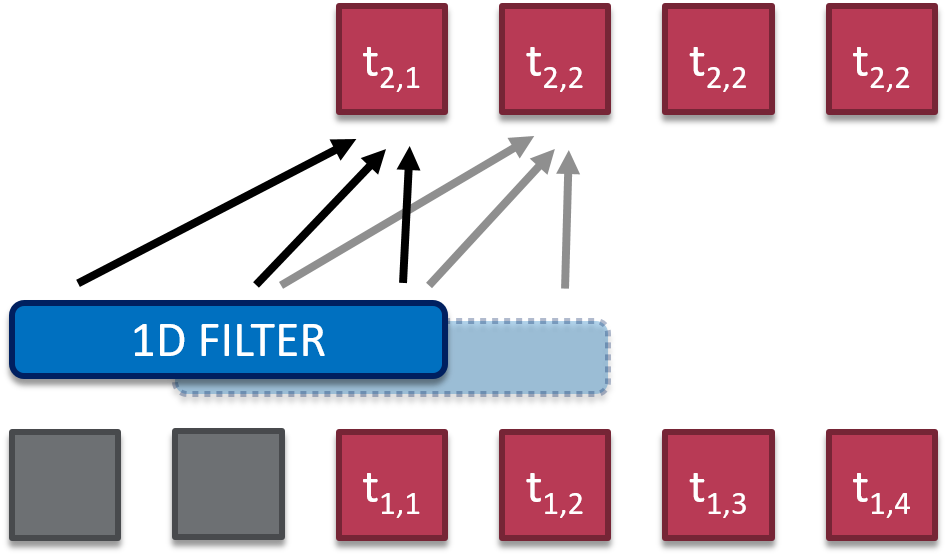
\includegraphics[width=120mm, keepaspectratio]{figures/1d-causal-conv.png}
	\caption{1D kauzális konvolúció paddinggel.}
	\label{fig:1d_causal_conv}
\end{figure}

\newpage

A \ref{fig:1d_noncausal_conv} ábra egy nem kauzális 1D konvolúciót mutat. A $t_{i, j}$ az i-edik rétegbeli j-edik neuron. Látható, hogy a $t_{2,1}$ jövőbeli időpillanatokból kap értékeket a szűrőn keresztül. Ennek megoldása a szűrő eltolása padding segítségéve. Ezt szemlélteti a \ref{fig:1d-causal-conv} ábra, ahol az egyes neuronok csak korábbi időpillanatokból kapnak értékeket. 

A beszéd generálásánál a \emph{t}-edik időpillanatban a hullámforma értéke a korábbi adatoktól függ. Ahhoz, hogy magas frekvenciájú, pl. 16 kHz frekvencián mintavételezett 
hangadattal tanítsuk a hálózatot nagy receptív mezőre van szükség. A receptív mező az a szélesség, amit a szűrő lát a bemenetből. 16 kHz esetén egy másodpercnyi jelet 16000 szám reprezentál. Ahhoz, hogy a hálózat helyesen jósolja meg a következő generált értéket, a hosszú távú dependenciákat figyelembe kell vennie, tehát a receptív mező méretét elég nagyra kell megválasztani. A probléma ekkora mezők esetén, hogy sok konvolúciós réteget igényelnek (egy korábbi időpillanatbeli adat plusz egy konvolúciós réteget igényel), ami növeli a számítási komplexitást. A nyújtott konvolúciók erre adnak hatékony megoldást. A filter meghatározott távolságokkal kihagy valamennyi inputot, majd figyelembe vesz egyet. Egymás utáni rétegekben a nyújtási tényezőt exponenciálisan növelve a receptív mező is exponenciálisan fog nőni.

\begin{figure}[!ht]
	\centering
	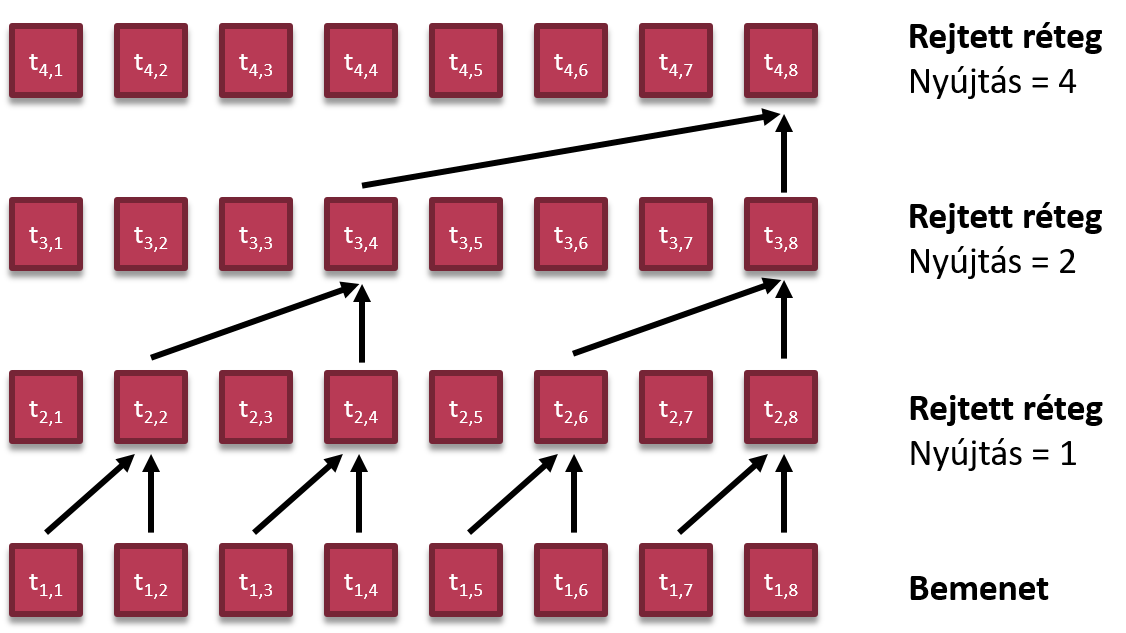
\includegraphics[width=150mm, keepaspectratio]{figures/1d-dilated-conv.png}
	\caption{1D nyújtott kauzális konvolúciós rétegek.}
	\label{fig:1d_dilated_conv}
\end{figure}

\subsubsection{SoftMax eloszlás}
A WaveNet SoftMax réteget használ a $p(x_t|x_1,\dots,x_t)$ feltételes valószínűségi eloszlás modellezésére.
Az audio jeleket általában 16 bites egészekkel kódolják, amelyek 65536 értéket vehetnek fel. Ebben az esetben a SoftMax rétegnek 65536 valószínűséget kell kimenetként adnia, melyek összege 1. A $\mu$-law kvantálást alkalmazva a beszédjel 256 biten kódolható és később az inverz transzformációval jó minőségben visszaállítható.

Az emberi hallás sokkal érzékenyebb alacsony amplitúdójú hangok kvantálási zajára, mint a magasabbakéra. Erre alapozva a $mu$-law kvantáló a jelet egy logaritmikus függvénnyel kvantálja úgy, hogy az alacsonyabb amplitúdójú jelek nagyobb felbontással (több bittel), a magasabbak pedig kisebbel lesznek kódolva. Ez növeli a SoftMax réteg hatékonyságát is, mert nagyobbak lesznek a valószínűségek közötti különbségek.

A tanítást a WaveNet klasszifikációs problémaként kezeli. A bemeneteket OneHot kódolással adjuk meg, a SoftMax réteg pedig az így kódolt egészekre ad valószínűségi eloszlást.

\subsubsection{Reziduális blokkok}

A WaveNet architektúra egymáshoz csatolt reziduális blokkokból és ún. kapcsolat-ugrásokból (skip-connection) épül föl. A reziduális hálózatok előnye, hogy orvosolják az elenyésző gradiens problémát, így sokkal mélyebb hálózat építhető.

\begin{figure}[!ht]
	\centering
	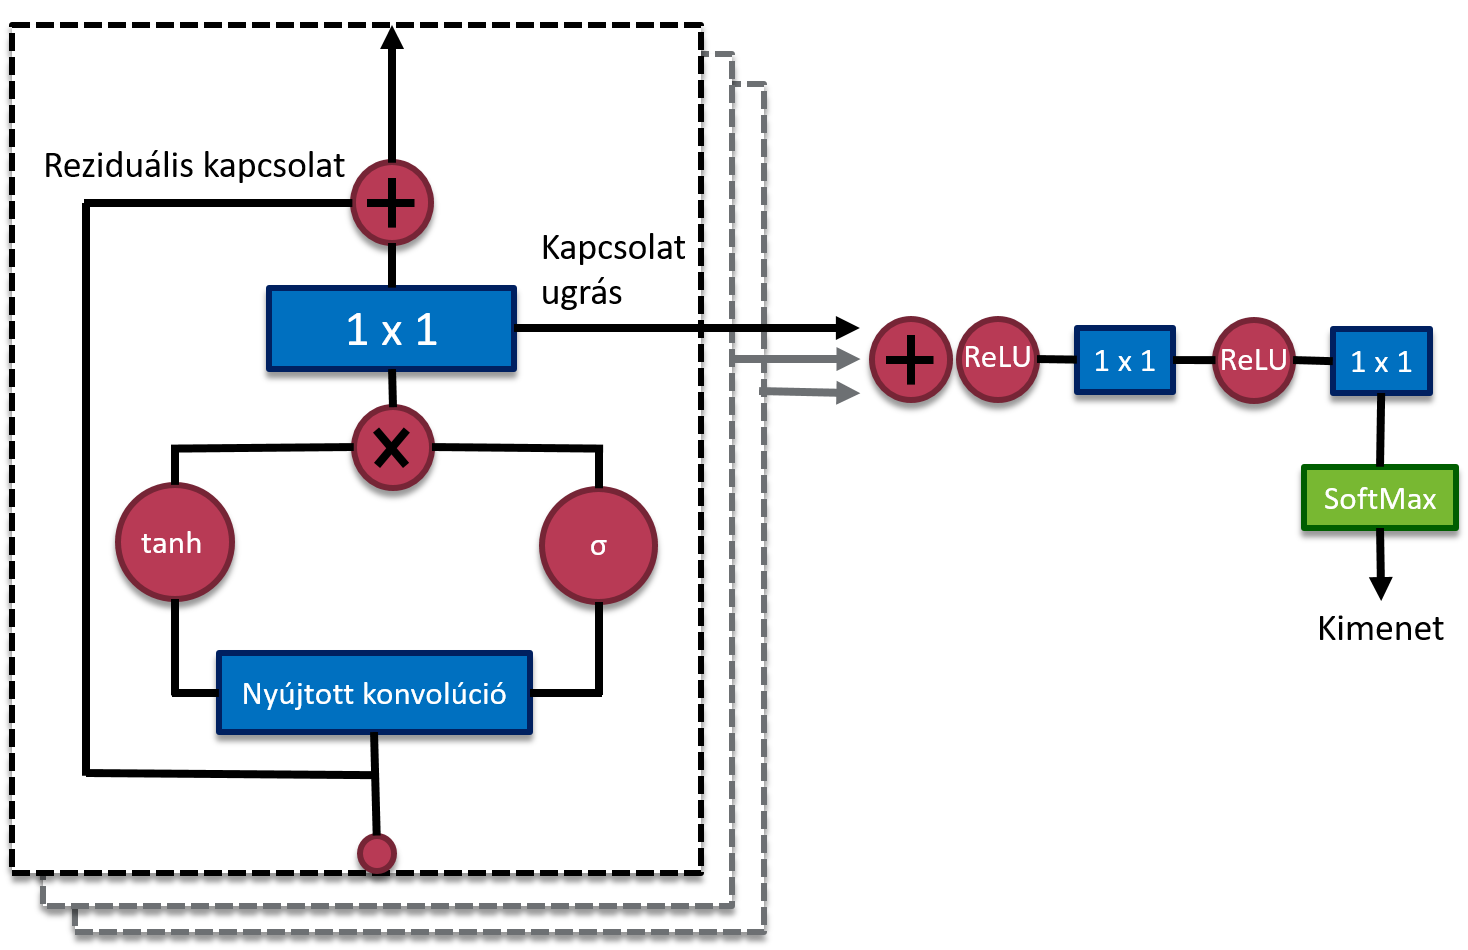
\includegraphics[width=150mm, keepaspectratio]{figures/wavenet_arch.png}
	\caption{WaveNet architektúra.}
	\label{fig:wavenet_arch}
\end{figure}

Egy reziduális blokk bemenete egy 2x1-es konvolúciós rétegen megy keresztül. Balra egy \emph{tanh}, jobbra egy szigmoid aktivációs függvényen haladnak át, majd elemenkénti szorzás és 1x1 konvolúció után egyrészt átugorja a reziduális kapcsolatot, illetve azzal együtt bemenetként szolgál a következő reziduális egységnek. Az 1x1 konvolúciós rétegek a dimenzionalitás változtatására szolgál. Külön 1x1 konvolúciós szűrők skálázzák a kimenetet a következő reziduális blokk bemenetére, és a kapcsolat-ugrásokhoz.

\subsection{Módosított WaveNet architektúra}

A módosított WaveNet architektúra segítségével a WaveNetet beszélőfelismerésre használhatjuk.
\bigskip
\begin{python}
	from WaveNetClassifier import WaveNetClassifier
	
	wnc = WaveNetClassifier((96000,), (10,), kernel_size = 2, dilation_depth = 9,
	                         n_filters = 40, task = 'classification')
	
	wnc.fit(X_train, y_train, validation_data = (X_val, y_val), epochs = 100,
	        batch_size = 32, optimizer='adam', save=True, save_dir='./')
	
	y_pred = wnc.predict(X_test)
	
\end{python}
\bigskip
A WaveNetClassifier objektum paraméterei:

\begin{itemize}
	\item \emph{input\_shape}: Bemeneti dimenziók tuple formájában. Például ha a bemenet egy 6 s hosszú hullámforma 16 kHz-en mintavételezve, a bemeneti dimenziók (96000,)
	\item \emph{output\_shape}: Kimeneti dimenziók tuple formájában. Például ha 100 osztály szerint klasszifikálunk, a kimeneti dimenziókból képzett tuple (100,).
	\item \emph{kernel\_size}: A konvolúciós filter/kernel mérete a reziduális blokkokban.
	\item \emph{dilation\_depth}: A reziduális blokkok száma.
	\item \emph{n\_filters}: A konvolúciós filterek száma a reziduális blokkokban.
	\item \emph{task}: Klasszifikáció vagy regresszió.
	\item \emph{regression\_range}: A regresszió céltartománya lista vagy tuple formátumban.
	\item \emph{load}: Előző WaveNetClassifier betöltése (bool).
	\item \emph{load\_dir}: A betölteni kívánt modell könyvtára.
\end{itemize}

\subsection{Eredmények}

A WaveNet classifiert mindkét beszédadatbázison teszteltem. A TIMIT beszédkorpusszal csak kevés beszélő esetén ért el jó eredményt, több mint 20 beszélő esetén a modell nem tanult. Ennek valószínűsített oka, hogy a TIMIT adatbázis beszélőnként 10 hangmintát tartalmaz.

\setlength\arrayrulewidth{0.6pt}

\begin{table}[!ht]
	\begin{tabular}{l|l} \toprule
		\bfseries Beszélők száma & 18 \\
		\rowcolor{gray!10}
		\bfseries Minta/beszélő & 100\\
		\bfseries Minta össz. & 1800 \\
		\rowcolor{gray!10}
		\bfseries Minta hossza & 4000 \\
		\bfseries Epochok száma & 43\\
		\rowcolor{gray!10}
		\bfseries Hiba & 0.0013 \\ 
		\bfseries Pontosság & 1.0 \\ 
		\bottomrule
		\hline
	\end{tabular}
	\centering
	\caption{Paraméterek CMU Arctic adatbázissal.}
	\label{fig:wavenet-arctic}
\end{table}

!!! teszthalmaz mérete !!!

Tanítás után a teszt adathalmazon a hálózat 96.799 \%-os pontosságot ért el.
\newline
\newline

A CMU Arctic adatbázisokat letöltöttem a Google Colaboratory-s fájlrendszerre és egy mappa alá mozgattam őket. Ehhez csak az adatbázis kódjára volt szükség, mindegyik azonos kezdetű url-en található.
A CMU Arctic 16 bit-es wav fájlokat tartalmaz. Normalizálásként minden mintavételezett értéket leosztottam a maximális hosszal ($2^15 + 1$), hogy 0 és 1 közötti értéket vegyenek fel.
\newline
\newline
Tanítómintáknak 2-3 másodperces részeket választottam. A megfelelő hosszú wav fájlokból kivágtam a [0:40000] részt, így pontosan $40000/16000 = 2,5$ s-os szeleteket kaptam. Mind a 18 adatbázisból kiválasztottam 100 ilyen mintát. Ezeket véletlenszerűen összekevertem és ez az 1800 elemű halmazzal tanítottam. Az epochok száma 200 volt, de mivel a tanítás a 43-44. epochnál már 1-es pontosságot és közel 0 veszteséget mutatott, leállítottam a folyamatot. 
\newline
\newline
\begin{figure}[!ht]
	\centering
	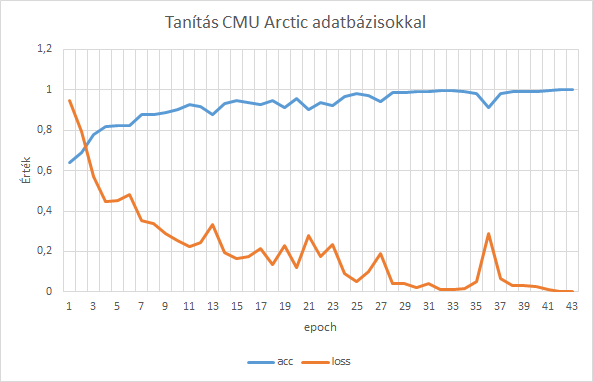
\includegraphics[width=150mm, keepaspectratio]{figures/wavenet-train-cmu-arctic.png}
	\caption{WaveNet tanítása CMU Arctic adatbázisokkal.}
	\label{fig:wavenet-train-cmu-arctic}
\end{figure}
\ \\
\newline
\newline

A teszthalmazba a tanítómintákon kívüli minimum 40000 hosszú wav fájlok kerültek, összesen 10152 minta.
Az elvárt kimeneteket one-hot kódoltam és kiértékeltem a modellt a tesztadatokon. A felismerés pontossága $97,3$ \% volt 18 ember esetén.

\section{SincNet}



\subsection{Eredmények}